% 11-07.tex
% FDG 2012 conference paper
% WORKS WITH V3.2SP OF ACM_PROC_ARTICLE-SP.CLS
% November 2011
% Author: George Lee, Yongwen Xu, Robert Brewer, Philip Johnson
%
% ----------------------------------------------------------------------------------------------------------------
% This .tex file (and associated .cls V3.2SP) *DOES NOT* produce:
%       1) The Permission Statement
%       2) The Conference (location) Info information
%       3) The Copyright Line with ACM data
%       4) Page numbering
% ---------------------------------------------------------------------------------------------------------------
% It is an example which *does* use the .bib file (from which the .bbl file
% is produced).
% REMEMBER HOWEVER: After having produced the .bbl file,
% and prior to final submission,
% you need to 'insert'  your .bbl file into your source .tex file so as to provide
% ONE 'self-contained' source file.
%

\documentclass{acm_proc_article-sp}

\begin{document}

\title{Makahiki: An Open Source Game Engine for Energy Education and Conservation}

%\numberofauthors{1} 

\author{
\smallskip
George E. Lee\\ 
\smallskip
Yongwen Xu\\ 
\smallskip
Robert S. Brewer\\ 
\smallskip
Philip M. Johnson\\
       \affaddr{Information and Computer Sciences}\\
       \affaddr{University of Hawai`i at M\=anoa}\\
       \affaddr{Honolulu, HI 96822}\\
       \email{[gelee, yxu, rbrewer, johnson]@hawaii.edu}
}

\maketitle
\begin{abstract}
  The rising cost, increasing scarcity, and climate impact of fossil
  fuels as an energy source makes a transition to cleaner, renewable energy
  sources an international imperative.  This paper presents Makahiki, an
  open source game engine for energy education and conservation.  Makahiki
  facilitates the implementation of ``serious games'' that motivate players
  to learn about energy issues, improve their intuition about the energy
  impact of appliances and behaviors, and enable them to discover how to
  use energy more efficiently in their normal life.  Makahiki has been
  used to implement ``The Quest for the Kukui Cup'', a three week energy
  challenge for over 1,000 first year students living in residence halls at
  the University of Hawaii in Fall, 2011.   Evaluation of this initial
  deployment of Makahiki has revealed useful insights into its game
  mechanics, ways to improve the next Kukui Cup challenge, and the
  challenges when adapting it to other energy contexts.
\end{abstract}

% A category with the (minimum) three required fields
\category{L.5.1}{Game-based Learning}{Gaming}

\terms{Human Factors, Games, Education, Motivation}

\keywords{Serious Games, Education, Gamification}% NOT required for Proceedings

\section{Introduction}

The rising cost, increasing scarcity, and climate impact of fossil fuels as
an energy source makes a transition to cleaner, renewable energy sources an
international imperative.  One barrier to this transition is the relatively
inexpensive cost of current energy, making financial incentives less
effective.  Another barrier is the success that electrical utilities have
had in making energy ubiquitous, reliable, and easy to access, thus
enabling widespread ignorance in the general population about basic energy
principles and trade-offs.  In Hawaii, the need for transition is
especially acute, as the state leads the nation both in the price of energy
(over \$0.30/kWh) and reliance on fossil fuels as an energy source (over
90\% from oil and coal).

Moving away from petroleum is a technological, political, and social
paradigm shift, requiring citizens to think differently about energy
policies, methods of generation, and their own consumption than they have
in the past.  Unfortunately, unlike other civic and community issues,
energy has been almost completely absent from the educational system. To
give a sense for this invisibility, public schools in the United States
generally teach about the structure and importance of our political system
(via classes like ``social studies''), monetary issues (though ``(home)
economics''), nutrition and health (through ``health''), and even sports
(through ``physical education'').  But there is no tradition of teaching
``energy'' as a core subject area for an educated citizenry, even though energy
appears to be one of the emergent issues of the 21st century.

Another emergent issue, at least for the first part of the 21st
century, is the explosive spread of game techniques, not only in its
traditional form of entertainment, but across the entire cultural spectrum.
The adoption of game techniques to non-traditional areas such as finance,
sales, and education has become such a phenomenon that the Gartner Group
included ``gamification'' on its 2011 Hype List, positioning it near the
summit of ``inflated expectations'' (after which it is projected to fall
into the ``trough of disillusionment''). 

This paper describes Makahiki, an open source game engine for energy
conservation and education, in which we attempt to create synergy between
these two emergent issues.  The result of over two years of research and
iterative development, Makahiki explores one section of the design space
where virtual world game mechanics are employed to affect real world energy
behaviors.  The ultimate goal of the Makahiki project is to learn how to
not just affect energy behaviors during the course of the game, but to
produce more long lasting, sustained change in energy behaviors and
outlooks by participants. 

We used Makahiki to create an energy challenge called The Quest for the
Kukui Cup for approximately 1,000 first year students living in the
residence halls at the University of Hawaii in Fall, 2011.  During the
three weeks of the competition, over 400 of the eligible students played
the game, for a total of 850 game play hours.  In addition to online play,
the Quest for the Kukui Cup integrated 24 real world events, including
workshops on energy-related matters, excursions to wind farms and other
energy related locations, and energy-related activities on campus. The game
mechanics were designed to create a self-reinforcing ``virtuous circle''
between the real world and virtual world activities.  The challenge was
very successfully received and plans are already underway to both repeat
the challenge in 2012 for University of Hawaii first year students, and 
adapt it to other residence halls and other universities in Hawaii.

The next section briefly reviews the research on which we based Makahiki
and the Quest for the Kukui Cup.   We then discuss the architecture and
game mechanics of the system, followed by the lessons we learned from its
first deployment. We conclude with our current goals for improvements to
the system.

\section{Related Work (Yongwen)}
Our research draws on work we've done previously
\cite{csdl2-11-03,csdl2-10-05,csdl2-10-07,csdl2-11-02}, as well as from
work done by others in the areas of energy behavior research, energy 
competitions, gamification and serious games. 

To reduce energy consumption, providing energy feedback is a critical 
foundation. Darby's survey of energy consumption studies from the past 3 
decades found  that, consumption in identical homes could differ in energy use 
by a factor of two or more depending on the behavior of the inhabitants
\cite{darby-review-2006}. Another survey of energy feedback conducted by 
Faruqui et al. found that residents that actively used the in-home displays 
with near-realtime feedback, averaged a 7\% reduction in energy usage
\cite{Faruqui09}. Darby also points out that feedback alone is not always 
enough, other factors such as training and social infrastructure could lead to 
higher rates of energy conservation\cite{darby-2000-making-it-obvious}.

Energy competitions or challenges have been introduced to college dormitories 
and residential homes as ways to incentivize energy reduction. Pertersen et 
al. describe their experiences deploying a real-time feedback system in an 
Oberlin College dorm energy competition in 2005 that includes 22 dormitories 
over a 2-week period\cite{petersen-dorm-energy-reduction}. Web pages were used 
to provide feedback to students. They found a 32\% reduction in electricity 
use across all dormitories. However, in a post-competition survey, respondents 
indicated that some behaviors, such as turning off hallway lights at night 
and unplugging vending machines were not sustainable outside the competition 
period.  Overall, there has been little analysis on energy usage after 
competitions finish, or how positive behavior changes could be sustained.

The Building Dashboard\cite{building-dashboard}, developed by Lucid Design 
Group, is used to support Oberlin's dorm energy competition,
as well as the Campus Conservation Nationals, a nationwide electricity and 
water use reduction competition on college campuses \cite{competetoreduce}. 
The Building Dashboard enables viewing, comparing and sharing building energy
and water use information on the web in compelling visual interface, but the 
cost of the system creates the barrier for wider adoptions. In additon, the 
building dashboard solutions focus on providing energy information as 
a passive media. There is little interaction between participants and the system.

Games on the other hand, have been shown with great potentials as a successful
interactive media that provide engaging interface in various serious 
contexts\cite{mcgonigal2011reality,reeves2009total}. Prebatch attempts to build
a game layer on top of the world with his location based service startup
\cite{Priebatsch2010ted}. 

Reeves et al. described the design of the Power house, 
a energy game that connect home smart meters to a online multiple player game 
with the goal to improve home energy behavior\cite{Reeves2011powerhouse}. 
In the game, the real world energy data is transformed from dull 
information into a "more palatable and relevant form of feedback", and players 
may be insentivized by the in-game rewards to complete more energy-friendly 
real-world behaviors. 

ROI Research and Recyclebank launched the Green Your Home Challenge as a case 
study of employing gamification\cite{Deterding2011mt} techniques online to 
encourage residential green behavioral changes offline\cite{gamingforgood}. 
Working with Google Analytics, the results show a 71\% increase in unique 
visitors and 97\% of participants surveyed say that the challenge increased 
their knowledge about how to help the environment. 

Blending of real and virtual worlds has been explored in broader contexts. 
Mcgonigal designed the award winning Serious Alternative Reality Game (ARG) 
"World Without Oil"\cite{worldwithoutoil} and later the "Evoke"
\cite{urgentevoke} game with the goal to help empower people to come up with
creative solutions to our most urgent real-world problems. ARGs have also been
used to support learning. Connolly et al. discuss the development of an 
Educational ARGs to motivate secondary school students across Europe to learn 
modern foreign languages\cite{connolly2009arguing}. The results of the pilot 
run of the game in 2009 indicated that 92\% of students felt the game had  
motivated students to learn a second language. One of problems
the team identified is the limitation of Moodle platform the game based on.

The report of the ARGOSI project provides insights to the use of ARGs in game
based learning and the challenges in the field of higer education
\cite{whitton2009alternate}. The pilot was run in University of Bolton with 
the aim to provide an engaging alternative to traditional methods of 
introducing students to university life. The overall up-take of the game was 
fairly low with 173 players and 23(13\%) of whom were active but the project
identifies number of questions surrounding educational ARGs, such as 
motivation, relationship to curriculum, marketing and timing. The report 
suggests that a complete ARG model may not be appropriate to be used in whole
for learning, and using game elements might have better potentials.

\section{System Design}
\begin{figure*}[t!]
  \center
  \includegraphics[width=0.5\textwidth, angle=90]{makahiki-architecture.eps}
  \caption{\em \small Architecture of Makahiki}
  \label{fig:MakahikiArchitecture}
\end{figure*}

Figure \ref{fig:MakahikiArchitecture} provides an overview of the different components of Makahiki and how they interoperate with each other. Section \ref{sys:Architecture} discusses the underlying technology of Makahiki and the 2011 Kukui Cup, while section \ref{sys:GameDesign} details the various games we implemented for the competition.

\subsection{Architecture}
\label{sys:Architecture}

The website is implemented using the Django web framework and the Python programming language. In addition to the modules we created, we used other third party libraries including ``django\_cas'' (an authentication plugin that allows users to log in through a CAS server), ``brabeion'' (a Django module for badges), ``minidetector'' (detects if a client is a mobile phone), and ``restclient'' (a library for interacting with RESTful web services). The website is hosted on a Xserve running Mac OS X Snow Leopard and Apache. To handle server loads more efficiently, we used memcached (an in-memory caching system) to cache parts of the website for quicker access.

We access another system called WattDepot for energy information.  WattDepot handles the storage of power data from the individual meters in the residence hall. However, calculating energy (power over a period of time) can be computationally expensive if we have to calculate it every time a user accesses a page. We implemented a ``cloud cache'' that uses Google Spreadsheets to store precomputed energy values for the different floors in the competition. The user's browser accesses the public spreadsheet using client-side javascript and the Google GData library. The server may access the cloud cache or WattDepot directly. For example, to award points in the energy goal game, a script is executed on the server once a day to check the daily energy goal spreadsheet and see if the individual lounges made their goal. Energy data for the floors over the past 30 days are also stored in a spreadsheet, so we can use client-side Javascript to compute the energy used during the competition.

\subsection{Game Design}
\label{sys:GameDesign}

During the course of developing Makahiki, we constructed several components and games for users in order to keep them more engaged. The following sections will discuss how each of these components and games contribute to the overall system.

\subsubsection{Rounds}

As part of the configuration for Makahiki, a competition period can be split up into rounds. The energy usage and points during a round are tracked separately but still contribute to the overall totals. If there is no round configured during the competition period, then the overall score is tracked. As an example, the 2011 Quest for the Kukui Cup was three weeks and had two week long rounds (round 3 was the overall round). This had the interesting side effect of putting the top players in round 1 in a slight disadvantage during round 2, since they have completed most of the tasks available to them. Players who are relatively new to the competition in Round 2 can complete tasks that were available in Round 1, although they do miss out on any events and excursions that happened during that time.

\subsubsection{Smart Grid Game}

\begin{figure}[h!]
  \center
  \includegraphics[width=0.5\textwidth]{smart-grid.eps}
  \caption{\em \small Smart Grid Game}
  \label{fig:SmartGrid}
\end{figure}

One of the primary components of Makahiki is the Smart Grid Game shown in figure \ref{fig:SmartGrid}. This is the primary place users go to to earn points in the competition. Tasks are organized into a grid of squares (hence the name ``Smart Grid'') and organized by category columns. There are 4 different types of tasks a user can complete in the Smart Grid; activities, commitments, events, and excursions.

Activities are the most basic task available in the Smart Grid. In order to get points for an activity, a user will have to provide a response to the administrators. These responses can be free response or an uploaded picture. Administrators can log in and access an admin page to approve or deny submissions. If a submission is approved, the user will receive the points for that submission. Otherwise, a user will be sent a website notification informing them that their submission was not approved. The user can change and resubmit their response and still earn the full point value for that task.

Commitments are pledges or declarations that the user will do something sustainable for a period of 5 days. Examples include reducing shower time, taking the stairs, and turning off the lights when you leave the room. Because these commitments are not verifiable, they are typically worth fewer points than activities. Furthermore, a user can only have up to 5 active commitments at any given time. After the 5 day period is up, the user can then declare that they completed the commitment. Once they do this, the points for the commitment are awarded immediately without any administrator approval. They can then sign up for another commitment, including the one they just completed.

Events and excursions are tied to real world activities. Events are held on campus while excursions take place off campus. Seating is limited, so users are asked to RSVP in advance. Users that do so are provided with a two point signup bonus. Users can also set up a reminder that is sent to their email and/or their mobile phone. Once the event or excursion takes place, an administrator will hand out attendance codes that can be redeemed on the website. These attendance codes are generated by Makahiki and can only be used once. To discourage users from signing up and not attending, a 2 point penalty is assessed to users who do not submit an attendance code. If the user submits an attendance code for the event after receiving this penalty, the penalty is reversed.

Not all of the tasks in the Smart Grid Game are necessarily available at the start of the game. We implemented a few predicates that can be used to determine if a task is locked or unlocked for a user. These predicates include:

\begin{itemize}
  \item Completed certain number of tasks within a category.
  \item Completed all tasks within a category.
  \item Completed certain tasks.
  \item Time-based unlocking (the task is available after a certain date).
\end{itemize}

These predicates are implemented using a limited subset of Python and can be changed within the Django admin interface. Competition designers can combine any of these functions in order to limit a user's path through the game.

\subsubsection{Daily Energy Goal Game}

\begin{figure}[t!]
  \center
  \includegraphics[width=0.5\textwidth]{daily-energy-goal-game.eps}
  \caption{\em \small Daily Energy Goal Game display on the energy page.}
  \label{fig:DailyEnergyGoal}
\end{figure}

Users are also provided with a daily energy goal. The goal for each floor is typically a percent reduction from their normal usage and is stored in a Google Spreadsheet. When a user goes to the energy page, they can view their current progress toward their daily energy goal. Near the end of the day, Makahiki checks the spreadsheet to see if a floor reached their goal. If the floor did reach their goal, each member of the floor that is participating in the game receives 20 points. 

Figure \ref{fig:DailyEnergyGoal} shows what a user would see when they go to the energy page. Note that the Daily Energy Goal display shows their current progress and their goal so far. We did this for two reasons. First, everyone will be under their actual energy goal for most of the day, so this display would not be very useful. Second, we have noticed that the students in the residence halls use more energy at night rather than during the day. Thus, it is easy to be under for most of the day and then jump over the goal at the very end. Displaying their goal so far provides a pace for users to follow. 

\subsubsection{Raffle Game}

\begin{figure}[t!]
  \center
  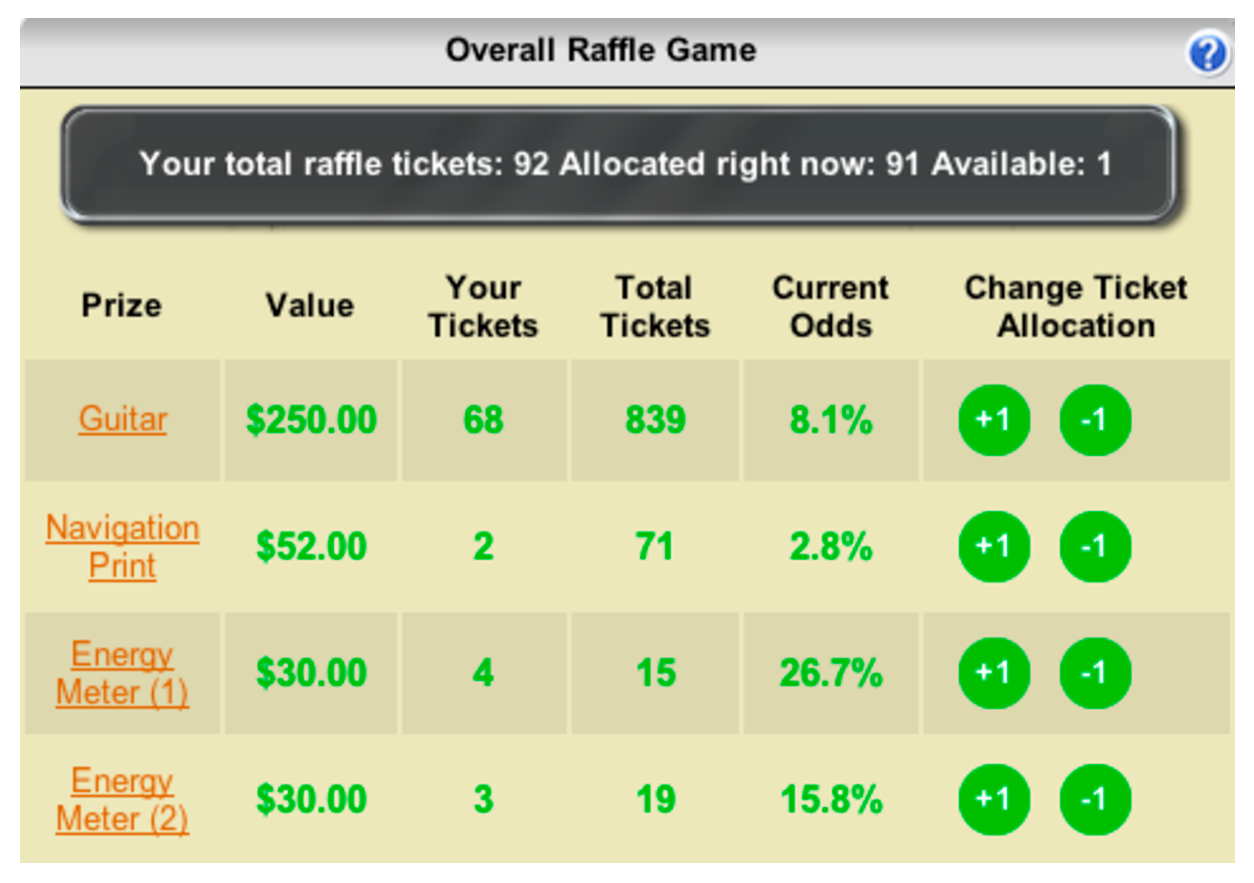
\includegraphics[width=0.5\textwidth]{raffle-small.eps}
  \caption{\em \small Raffle Game for the Overall Round}
  \label{fig:RaffleGame}
\end{figure}

In addition to the prizes for the individual and residence hall floor points and energy leaders, players can also earn prizes through the Raffle Game. Every 25 points in a user's overall score earns them one raffle ticket. A user can then add or remove their tickets from each raffle prize. Each round of the competition has their own set of raffle prizes and any unused raffle tickets carry over to the next round. It is also important to note that raffle tickets are independent from their score; using a raffle ticket does not affect their rank. Figure \ref{fig:RaffleGame} shows the Raffle Game during the last overall round of the 2011 Kukui Cup.

\subsubsection{Social and Referral Bonuses}

In an effort to get people to get friends or floor members to participate in the competition, we implemented two types of bonuses; social and referral. The social bonus is an administrator option when a task is created in the Smart Grid Game and awards extra points if the user has done the task with someone else. Examples of tasks that could be done with others include going to an event, recording a song related to energy, or decorating a door. When a user submits a response for a task with a social bonus, they have the option of providing the email address of the person they did it with. Then, once the other person submits their response, both users receive the social bonus. Social bonuses are not bi-directional; if the second user doesn't provide the first user's email address, they will still both get the social bonus.

When a user logs in to Makahiki for the first time, they are taken through a setup process. One of the steps in this process is the referral bonus. If  a user was referred by another user in the system, they can use this step to input their email address. Then, once the user earns 30 points in the competition, both users are awarded a referral bonus of 10 points. Typically, going through the setup process gives you 25 points, so we wanted to encourage the new user to at least complete another task in order to get the referral bonus.

\subsubsection{Quest Engine}

The main challenge we faced when designing Makahiki was providing adequate help to the user. We want the website to be intuitive, but a new user coming to Makahiki probably does not know what to expect. This is unlike most web applications, like Gmail, where the user has a specific task that they wish to accomplish. In an effort to provide a user with guidance through Makahiki after the setup process, we implemented the Quest Engine. Quests are used to guide the user through the various workflows of the site, like completing a task, signing up for an event, or allocating a raffle ticket. These quests can be created in the admin interface and also use a set of predicates to determine unlock and completion conditions. These predicates are:

\begin{itemize}
  \item Participating in a task or type of task.
  \item Completed a task or type of task.
  \item Has a certain number of points (in a round or overall).
  \item Completed a certain number of tasks in a category or of a given type.
  \item Awarded a badge.
  \item Wrote a post on their floor wall.
  \item Added a picture to their profile.
\end{itemize}

\subsubsection{Canopy}

\begin{figure}[t!]
  \center
  \includegraphics[width=0.5\textwidth]{canopy-missions-visualizations.eps}
  \caption{\em \small Canopy Missions and Visualizations}
  \label{fig:CanopyMissions}
\end{figure}

We designed the Canopy to be a place for the top users of the competition to go and view more advanced energy visualizations and tasks. The current visual design of the system has a forest background with trees, bushes, and grass. The Canopy got its name because it is a level above this forest level. The background of the canopy is actually different from the rest of the system, with tree tops on the bottom and blue skies on top. Players need to be invited to the canopy; it is not available to just anyone. A competition administrator runs a command on the server that adds the top n users to the Canopy.

In addition to the new background, the Canopy page includes new components. First, there is a Canopy wall that members can use to communicate with other Canopy members as well as administrators (who can always access the Canopy). Second, there are Canopy missions that replace the quest interface. Unlike quests, missions do not use predicates in order to determine when they are completed. Instead, missions are completed when their related Canopy tasks are completed. These Canopy tasks are based on the tasks in the Smart Grid game, but they do not appear in the Smart Grid. Also, some Canopy tasks may require collaboration with others instead of it being optional. Finally, the Canopy includes advanced energy visualizations, which give members additional insight into how the other floors are doing in the energy competition. Unlike the energy data displayed on other pages, these advanced energy visualizations access WattDepot's API directly. Figure \ref{fig:CanopyMissions} shows an example of a mission and an advanced energy visualization.

When we designed the Canopy, we initially thought we would provide points for completing Canopy tasks. However, because of the invitational nature of the Canopy, we wanted it to be fair to users who are not in the Canopy. The Canopy should not look like a way for the Canopy members to separate themselves from the rest of the users. Thus, instead of points, Canopy tasks award ``Canopy Karma''. A scoreboard is shown on the Canopy page and the top member earns a prize.

\section{Lessons Learned}

Our initial deployment of Makahiki for the 2011 Kukui Cup yielded many
useful lessons for next year's Kukui Cup as well as for others wishing to
implement serious games for energy. 

These lessons derive from both qualitative and quantitative sources of data
regarding the system.  First, as noted above, Makahiki provides custom quantitative
instrumentation that enables us to track when, where, and for how long each
user accessed each page of the site.  Unlike generic logging infrastructure
like Apache Web Stats, we could track application-specific behaviors. For
example, our instrumentation enables us to determine how users allocated
and deallocated tickets to the Raffle Game, or whether they watched,
paused, or skipped over the video portion of a Smart Grid Game activity.

Second, we gathered quantitative data through a survey that players could
complete as part of a Smart Grid Game activity during the final week of the
competition. The survey asked participants to provide short, free text
answers to questions regarding the way the competition and website was
designed.   41 players completed this survey.

These two forms of data enabled us to gain insight from active players of
the game.  However, they do not provide insight into the reasons why
certain students decided not to play the game.  We contacted a random
sample of students who chose not to play the game for interviews in order
to obtain some partial understanding of this portion of our population.

\subsection{Lesson \#1: Focus groups and usability evaluations improve player
  experience.}

Somewhat unintentionally, our experience with Makahiki has provided an
example of the benefits of focus groups and usability evalutions in game
design, as well as the costs of not doing so.  We spent almost an entire
year on an iterative design process for the main portions of the site which
included extensive end-user involvement.  We performed an interface
usability study with paper prototypes, two rounds of individual user
evaluation of the onboarding experience, and a beta test with a small
number of ``friends and family'' users prior to deployment.

Both qualitative and quantitative data indicate that the portions of the
game resulting from this process were successful.  In response to a survey
question asking how the player might describe the Kukui Cup, 83\% said
``Fun'', 95\% said ``Educational'', while 7\% said ``Difficult'' and 2.3\%
said ``Boring''.  In response to the question, ``What was confusing in the
website'', 46\% of the players said ``Nothing'', and 32\% of the users also
responded ``Nothing'' in response to the question, ``What would you change
about the website? When asked what they liked most about the website, 60\%
of the survey respondents said ``ease of use''.

Instrumentation also indicates that the game was generally easy to
use. 73\% of the 418 players never accessed the ``Help'' page, and only 5\%
of the users sent a question to the administrators. 

On the other hand, we designed and implemented the ``Canopy'' level of the
game in a very short period prior to the deployment, with no time available
for user evaluation and iterative design.  The results for the Canopy
level, both qualitative and quantitative, provide a stark contrast to the
main portions of the site.  We provided access to the canopy to the top
10\% of the players during the third round, and out of these 41 players,
only 11 spent more than 10 minutes in the Canopy, and only 5 spent more
than 30 minutes. These same users spent an average of 15 hours playing the
overall game.  Qualitative feedback indicated that we made several game
design errors in the Canopy that led to reduced player motivation and
interest in this part of the site.  We believe that these problems could
have been found and avoided if we had conducted user evaluations for this
part of the site prior to deployment.  As it is, we will make these
corrections for the 2012 Kukui Cup.

Although focus groups and usability evaluation tend to be viewed as
``motherhood and apple pie'' in software engineering, the Mahahiki game
development experience provides significant evidence for the improved user
experience that results from their use, as well as the costs that result
when schedule pressure forces deployment without them.

\subsection{Lesson \#2: Serious games require serious marketing.}

The Kukui Cup achieved a relatively high adoption rate: out of the 1035
residents who were eligible, almost 40\% played the game.  This is an
impressive adoption rate, both from the perspective of residential life
administrators (who rarely succeed in designing a residence hall activity
that gets nearly half of the students to engage with it) and from the
perspective of university energy challenges (where adoption rates of
10-15\% are more common.)  

On the other hand, our qualitative and quantitative data indicates that
there is substantial room for improvement, and that the single biggest
improvement opportunity identified by the players is better marketing.  In
response to the survey question asking how to improve attendence at real
world events, 60\% of the students suggested improved marketing and/or email
announcements as the best way to improve attendance.  Only 5\% indicated
that the actual events, as opposed to the way they were advertised,
constituted the major problem.

Our attempts at marketing the inaugural Kukui Cup at times resembled a
comedy of errors. For example, to kick off the challenge, our graphic
design intern designed a series of large (2 foot by 5 foot) banners to be
hung in the lobby of each of the four towers as the challenge progressed.
These banners were attractive---so attractive that the first set of banners
for all four towers were stolen in the middle of the night within the first
three days after we hung them up.  After this happened, we requested that
the second set of banners for the four towers be displayed only when staff
was on duty to monitor them.  This request resulted in only three of the
second set of four banners being stolen: the fourth being spared because
the on-duty staff never remembered to display it.  For next year, we hope
to create display materials that are ``cool, but not too cool''.

On a more positive note, game mechanics like the ``viral marketing''
referral bonus appeared to work well, with over XX students trying out the
site as a result of encouragement from other students.  


\section{Future Directions}

We are already planning the 2012 Kukui Cup, and our efforts are encouraged
by the fact that 98\% of the students in our survey said they would play
the Kukui Cup again next year if they could. 

We will, of course, focus more energy on marketing, and our goal is to
increase participation from 418 players to at least 600, which would
achieve the highest adoption rate of any dorm energy challenge of this
type.  We intend to harness the energy of this year's top players to
support and encourage participation from next year's first year students.

We remain convinced that the Canopy page, with its emphasis on advanced
energy visualizations and analyses, has the potential to provide a rich educational
opportunity to motivated students 



\section{Acknowledgments}

Makahiki has been supported in part by grant IIS-1017126 from the National
Science Foundation, and by funding from the University of Hawaii Office of Facilities
Management.   We gratefully acknowledge the 418 players of the 2012 Kukui
Cup and the members of the Kukui Cup team in addition to the authors who made the vision a
reality:  Kaveh Abhari, Hana Bowers, Greg Burgess, Caterina Desiato,
Michelle Katchuck, Risa Khamsi, Alex Young, and Chris Zorn. 

\bibliographystyle{abbrv}
\bibliography{csdl-trs,gamification,sustainability}  

\balancecolumns

\end{document}
